\section{Discussion}\label{sec:discussion}
\subsection{Task 1}
The first resonant frequency in the 1 mm grid spacing occurs at 11.502 GHz and in the 0.5 mm grid spacing it occurs at 11.4572 GHz (Figure \ref{fig:freqresponse1mm}). The amplitude is lower than in the examples in the lab manual due to the fact that we placed the probe off-centre in the structure. This way some of the different resonant frequencies cancel each other to lower the amplitude. However, the position of the resonant frequencies is preserved. Resonant frequency data is summarized in Table \ref{table:resolution}.

\begin{figure}[tbph]
\centering
\includegraphics[width=0.95\linewidth]{"graphics/freq response 1mm"}
\caption{Time and frequency response of excitation by magnetic pulse in 1.0 mm resolution cylindrical cavity. Starting in the upper right and proceeding counter-clockwise: I shows the impulse excitation; II shows the time response of $H_z$; III shows the frequency response of $H_z$, and; IV shows the bottom of the cylinder, the animation plane, probe and source.}
\label{fig:freqresponse1mm}
\end{figure}

\subsection{Task 2}
The third, fourth and fifth resonant frequencies in the 0.5 mm resolution are quite different from the ones in the 1 mm resolution. This is possibly due to the fact that the cavity looks significantly more circular at 0.5 mm, than it does at 1 mm. As the resolution approaches 0 mm the geometry of the discretized volume approaches the ideal cylinder. The ideal cylinder is maximally (infinitely) symmetric along the cardinal axes and the degree of symmetry contributes to the maximum magnitudes of the resonant frequencies.

\begin{figure}[tbph]
\centering
\includegraphics[width=0.95\linewidth]{"graphics/freq response 05mm"}
\caption{Time and frequency response of excitation by magnetic pulse in 0.5mm resolution cylindrical cavity. Starting in the upper right and proceeding counter-clockwise: I shows the impulse excitation; II shows the time response of $H_z$; III shows the frequency response of $H_z$, and; IV shows the bottom of the cylinder, the animation plane, probe and source.}
\label{fig:freqresponse05mm}
\end{figure}

\begin{table}[htpb]
	\centering
	\caption{Effect of mesh resolution on resonance frequency and magnitude}
	\label{table:resolution}
	\begin{tabular}{@{}SSSS@{}}
		\toprule
		\multicolumn{2}{c}{1 mm} & \multicolumn{2}{c}{0.5 mm} \\ 
		\multicolumn{1}{c}{Frequency (GHz)} & \multicolumn{1}{c}{$\left|F(f)\right|$} & \multicolumn{1}{c}{Frequency (GHz)} & \multicolumn{1}{c}{$\left|F(f)\right|$} \\ \midrule
		11.502347 & 9.4783414 & 11.457286 & 9.5471305 \\
		18.388106 & 2.1604907 & 18.341709 & 2.0439611 \\
		26.447574 & 6.3284078 & 26.38191 & 4.8253084 \\
		33.568075 & 6.5797428 & 33.567839 & 4.827887 \\
		41.314554 & 10.81526 & 41.2586281 & 12.360819 \\ \bottomrule
	\end{tabular}
\end{table}

\subsection{Task 3}
In order to have accurate results from a numerical reading, it is important to have an idea of what the actual value should be. It is easy to get very precise readings that are very inaccurate. One way to know if the measurement is accurate is by comparing it to a known value. Comparison to a forecast or calculation of what it should be can also help with determining accuracy. Resolution varies directly with accuracy but inversely with computation time (as observed in the lab, 0.5mm took longer to run than 1.0 mm).

\subsection{Task 7}
The curves of \texttt{int\_E\_dot\_dL.txt} and \texttt{d\_int\_B\_dot\_dS.txt} overlap completely (Figure \ref{fig:faraday}). Variances could be caused by the way the derivative is taken. If the time steps are large, they could miss an important piece of information. This would cause the two graphs to look different. 

\begin{figure}[tbph]
\centering
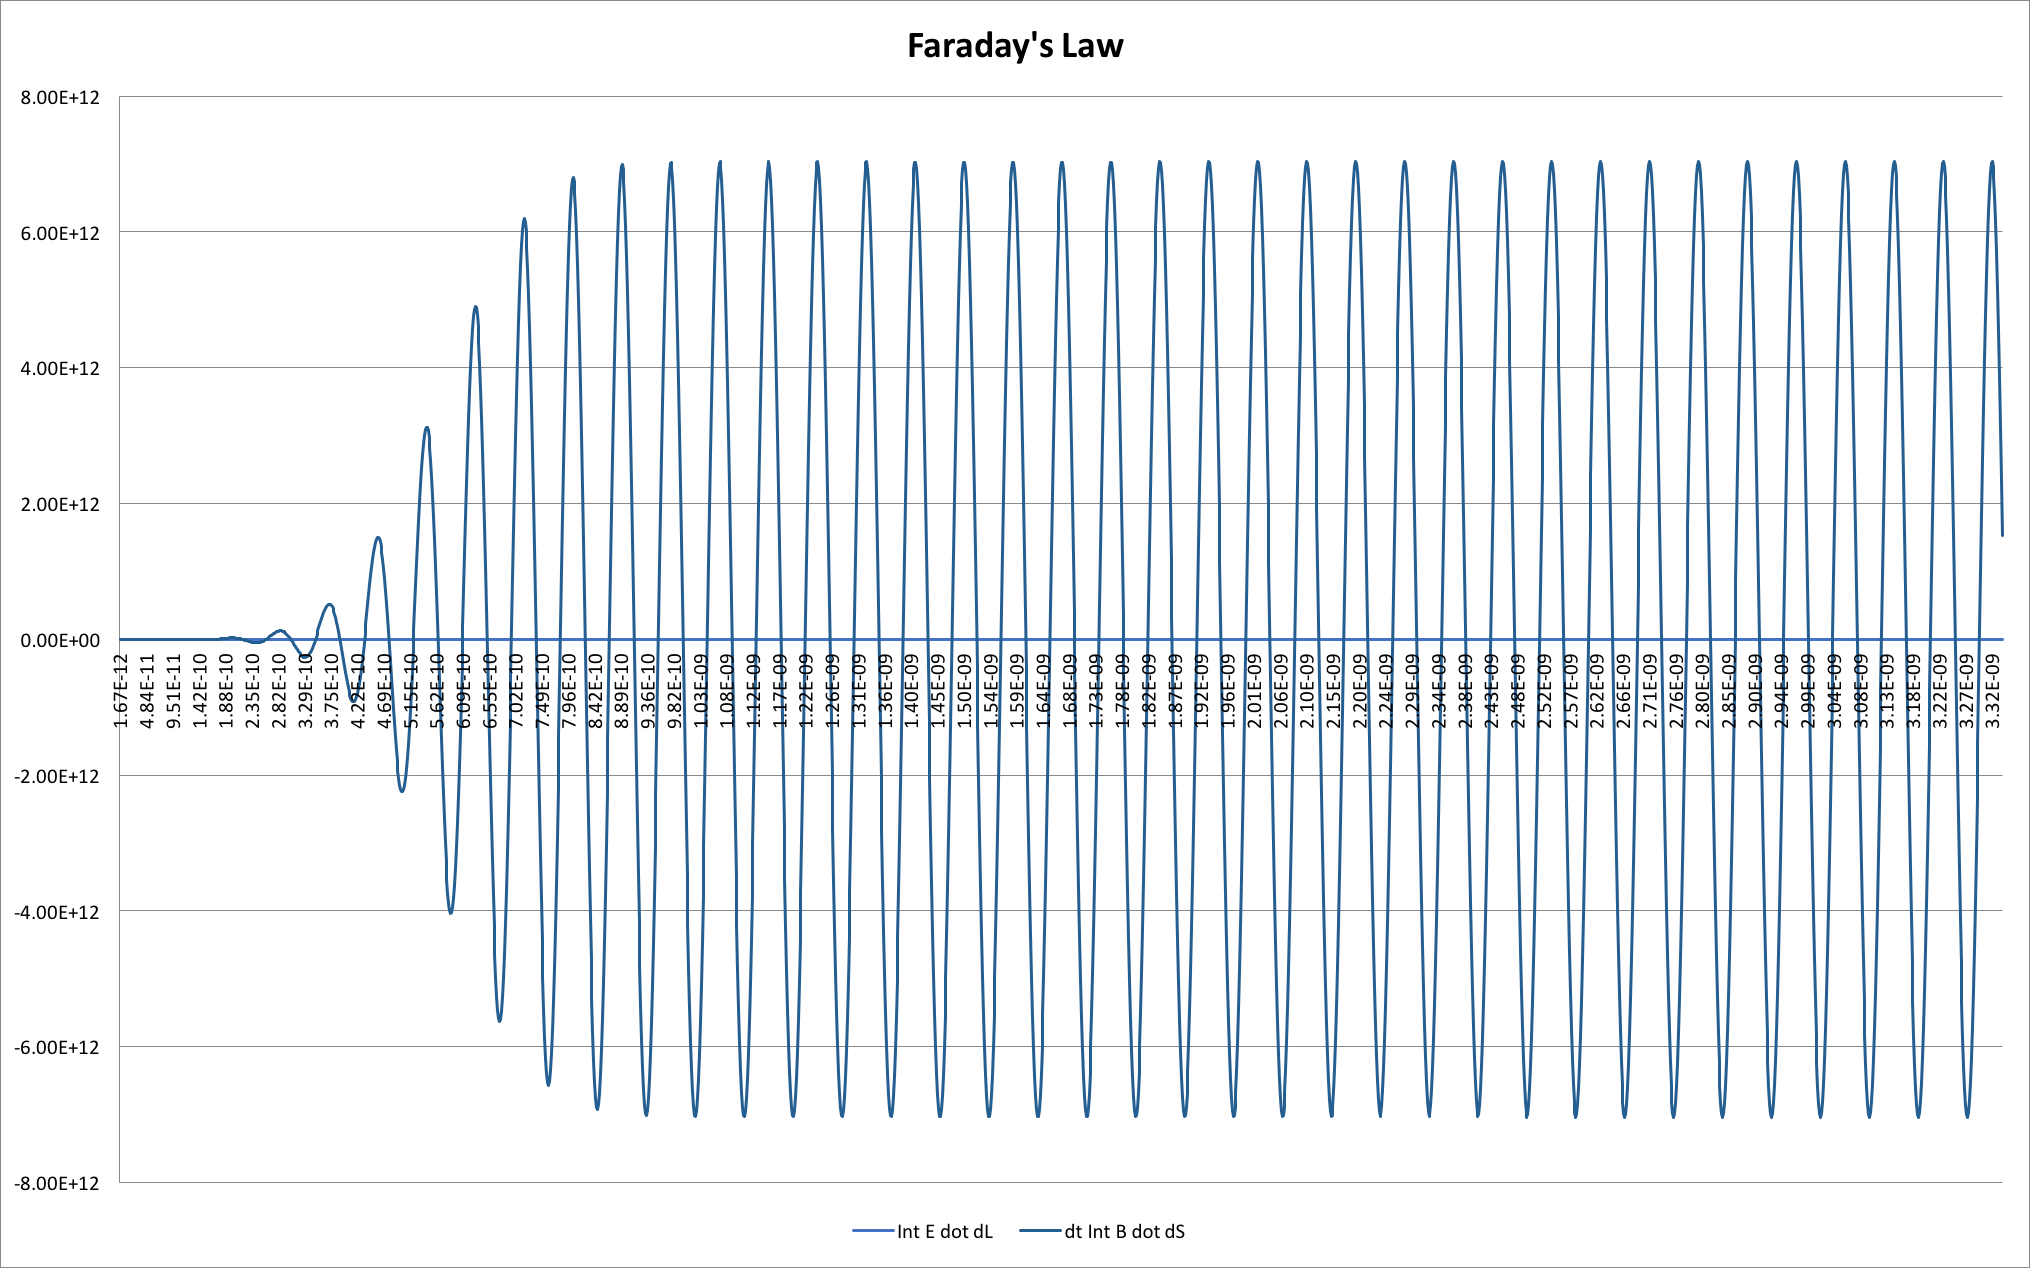
\includegraphics[width=0.95\linewidth]{graphics/faraday}
\caption{Complete overlap of $\eDOTdl$ and $-\bDOTds$}
\label{fig:faraday}
\end{figure}

\subsection{Task 10}
The curves of \texttt{int\_H\_dot\_dL.txt} and \texttt{d\_int\_D\_dot\_dS.txt} overlap completely (Figure \ref{fig:ampere}). Variances could be caused by the way the derivative is taken. If the time steps are large, they could miss an important piece of information. This would cause the two graphs to look different. 

\begin{figure}[tbph]
\centering
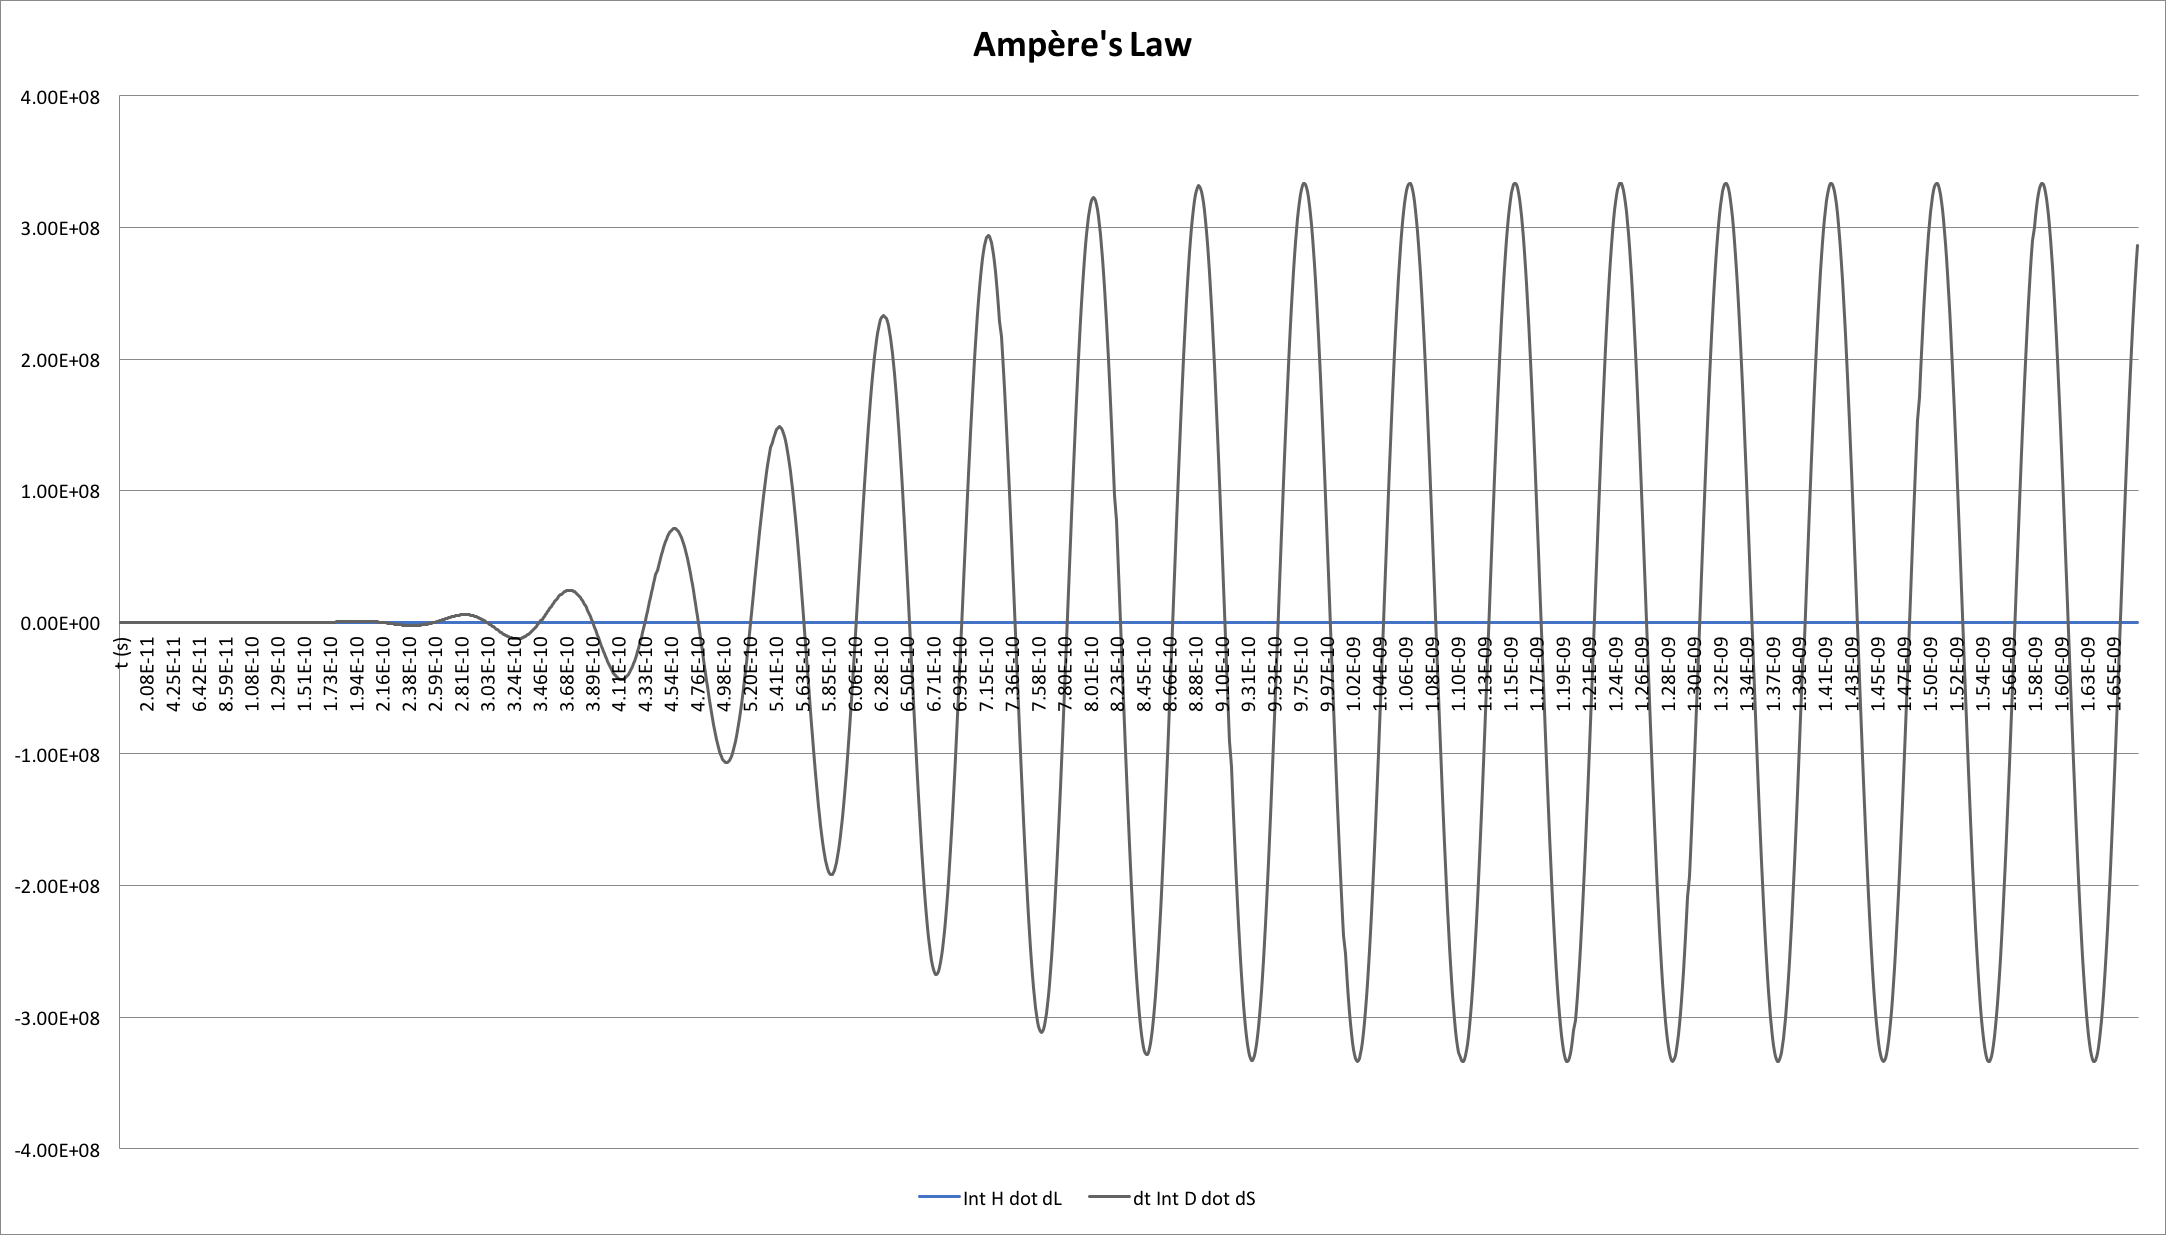
\includegraphics[width=0.95\linewidth]{graphics/ampere}
\caption{Complete overlap of $\hDOTdl$ and $\dDOTds$}
\label{fig:ampere}
\end{figure}



